\chapter{Design}

Current storage systems secure data either via encrypting data on the wire, or through data encryption on the physical disk\cite{ErikRiedelMaheshKallahalla2002}. Cryptographic protection of single file instances could prevent data modification or leakage during storage\cite{Vaquero2010}. Secure Dropbox is designed as a client end encryption tool over the Dropbox service. The main idea is providing a file encryption service with symmetric cryptography where key is not known to Dropbox and, in the meantime, the file encryption key is well protected with asymmetric cryptography for secure file sharing. It is proposed to strengthen the way in which the Dropbox protects users’ file content security from attacks especially those from internal Dropbox. Internal attack is theoretically easy to be performed as Dropbox encrypts those files with keys known to them. Also the security against external attack has been fortified since files will be encrypted twice, Dropbox and Secure Dropbox respectively. Secure Dropbox is proposed to be a C/S architecture system. The server end will work as a key management service (KMS) which mainly processes key management requests and storage request while the client end running on a user's host computer will perform cryptographic computations which are resource consuming. Secure Dropbox performs file operations like uploading, downloading and sharing via Dropbox API or the Dropbox official client which is essentially built with Dropbox API as well. The user interface of Secure Dropbox will be designed as a file system operation interface. Encryption within this service will be transparent to the users. The very security of Secure Dropbox service is based on user’s proper usage of Secure Dropbox account information. Two application modes will be provided: using regular mode when there is Internet access while in local mode when there is no Internet access. The different operation permission schema is granted to users.

\begin{figure}[h]
        \centering
        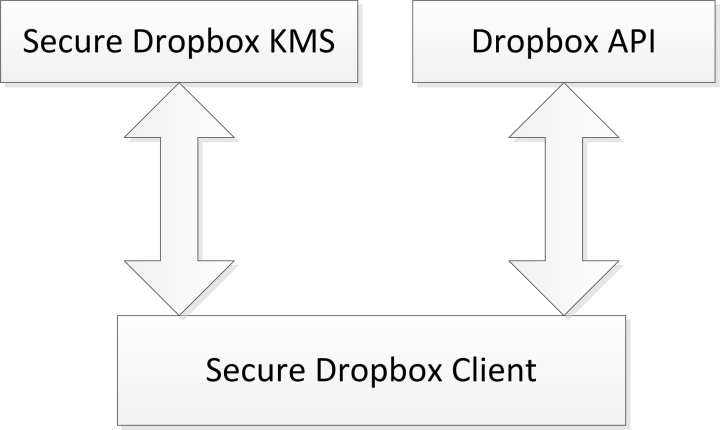
\includegraphics[width=0.6\textwidth]{figures/Secure_Dropbox_Architecture.png}
        \caption[Secure Dropbox Architecture] {Secure Dropbox Architecture}
\end{figure}

This chapter will discuss some major design decisions and implementation challenges during the Secure Dropbox project. Firstly, the overall design of Secure Dropbox will be proposed. Secondly, the cryptography application mechanism to guarantee the security of Secure Dropbox will be explained and justified. Furthermore, the reason for making choices about ways of performing file operations, systematic integration with Dropbox and a platform on which to construct the application will be discussed in regard to building a platform independent application. Moreover, the decisions made in terms of building a C/S architecture application but not in B/S architecture will be explained. Some other design features are more intuitively understandable by explaining from the implementation aspect so more detail of those parts will be proposed in the next chapter or just briefly mentioned in this chapter. Lastly, the design decisions and other principles proposed to implement Secure Dropbox are not Dropbox oriented specifically but could be adopted when designing any application that protect users file in the cloud and provide a reliable file sharing in the cloud storage system.

\section{Application of Cryptography}

Dropbox claim that they are using Secure Socket Layer (SSL) on data transmission and performing AES 256-bit encryption with users’ data. It seems sufficient against external attack but only on condition that the attacking does not come to key management service (KMS). However, these mechanisms make no sense of protecting users’ data from internal attack, which is performed by employees of Dropbox who have access permission to KMS. The behavior, or say the ability, of accessing to users’ data has been admitted in their terms of service\cite{Dropbox2012} that Dropbox will remove the encryption from file data and deliver them to law enforcement on government’s requirement. Nevertheless, because of internal attacker’s proficient understanding of Dropbox system and some inappropriate access permission configurations, internal attacks could even be done unconsciously. These security concerns have been certified that several internal attack events are reported. Client end encryption is one of those alternatives recommended by Dropbox if users are more willing to conceal their data and care less about losing some Dropbox features like version control or data recovering\cite{Dropbox2012}. More importantly, when protecting user’s data from internal Dropbox attack with client end encryption, it actually disables the file sharing infrastructure provided by Dropbox totally.

Anyway, cryptography is still going to be the very insurance for the security of Secure Dropbox. Generally, Secure Dropbox is designed to make Dropbox internal attack impossible and also to provide a cipher file sharing service. To achieve this goal, Secure Dropbox will apply a combination of symmetric cryptography and asymmetric cryptography. The symmetric cryptology like AES or DES will be used for file content encryption given the fact that they are much faster than asymmetric cryptography and sufficient security offered. The asymmetric cryptology is used for protecting the symmetric encryption key and providing a secure key transmission service. In the following example, the procedure of secure storage is going to be illustrated with AES and RSA as instance of symmetric and asymmetric cryptography respectively:

\begin{figure}[h]
        \centering
        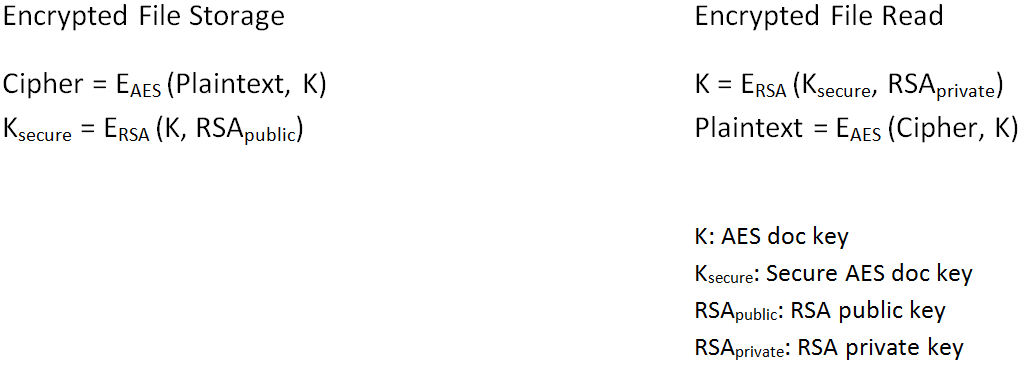
\includegraphics[width=1.0\textwidth]{figures/Encrypted_File_Storage_&_Reading.png}
        \caption[Encrypted File Storage and Reading] {Encrypted File Storage and Reading}
\end{figure}

In the file encrypted storage procedure, plain text is ciphered in AES with a random generated AES file encryption key. The doc key is later ciphered in RSA as well with file owner’s RSA public key.
In encrypted file read procedure, firstly the ciphered doc key $K_{secure}$ should be deciphered in RSA with file owner’s RSA private key. Having retrieved the raw doc key K, the cipher could be decrypted in AES with K.
The procedures of sharing from Secure Dropbox users is mainly about ciphering the doc key K and transferring it to the sharing recipient. K should be ciphered by file owner but could only to be deciphered by sharing recipient, which is a typical scenario for asymmetric cryptography application. In the following example, Alice wants to share a file with Bob:

\begin{figure}[h]
        \centering
        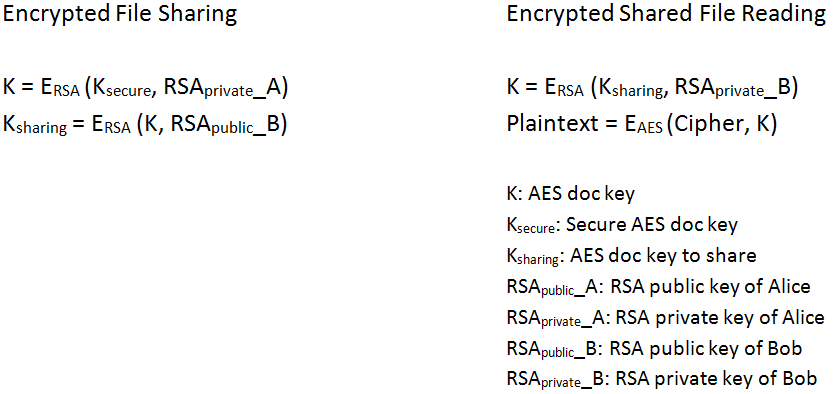
\includegraphics[width=1.0\textwidth]{figures/Encrypted_File_Sharing.png}
        \caption[Encrypted File Sharing] {Encrypted File Sharing}
\end{figure}

Sharing procedure as shown above actually does not perform any operation on the file instance but only cipher the key for sharing purpose. The doc key is stored in a secure way at the very beginning. To get the raw doc key, Alice has to decipher $K_{secure}$ in RSA with her own RSA private key. In order to enable Bob deciphering the key ciphered by Alice, she should encrypt the raw doc key K in RSA with Bob’s RSA public key, which is open to all the users in the Secure Dropbox system. $K_{sharing}$ is generated in this way and then transmitted to Bob via secure tunnels. After receiving the $K_{sharing}$, Bob will decrypt it in RSA with his own RSA private key and then get the raw doc key. Now the plain text of the shared encrypted file could be retrieved by decrypting in AES with the raw doc key.

Respecting managing the RSA key pair of Secure Dropbox user and doc key of each file, a detailed design description will be given in the coming section.


\section{Key Management Service}

In the Secure Dropbox application scenario, there should be an infrastructure posting all Secure Dropbox users’ RSA public key for sharing sponsor to achieve during the encrypted file sharing procedure. In addition, given the essence of Secure Dropbox (a client end file encryption tool) and Dropbox’s cloud storage nature, the requirement of everywhere use should be met. It means as long as users could get access to Dropbox, they are allowed to use the Secure Dropbox service like downloading the desired doc key chain and RSA key pairs. To achieve the goal, besides generating a local copy of essential data like Secure Dropbox users’ authentication information, RSA key pairs, doc keys and file sharing information, these records should also be stored on a server which is able to be accessed anytime anywhere.

Dropbox stores file encryption key in its own database makes it not an accredited storage service to users. However, in order to avoid same security concerns towards Dropbox about its encryption mechanism, some improvements should be made. To make Secure Dropbox reliable, the authority of decrypting file should be only granted to owner but no one else even the KMS administrator. A possible alternative is storing all sensitive data (e.g. RSA private key and doc key) on the server confidentially so that the everywhere usage could be realized safely. Therefore, the only entry (assume it could be something like an access token or password) of decrypting all these sensitive data should never be stored on the server but only held by users themselves.

\begin{figure}[h]
        \centering
        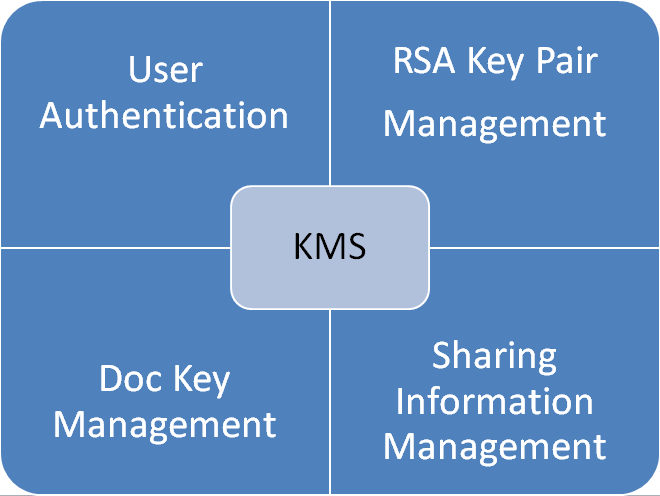
\includegraphics[width=0.6\textwidth]{figures/KMS_Architecture.png}
        \caption[KMS Architecture] {KMS Architecture}
\end{figure}

\subsection{KMS User Authentication}

User authentication information is a basic component in any web application instance as long as access control is required. The classic way applied in web application saves user’s authentication could be adopted: for the minimum usage, a plain text username and a hashed password should be saved. The authentication procedure will match the username and password hash value. The hashed password is generated in the client and only the hash value with algorithm indicator prefixes will be uploaded to KMS and stored. To avoid performing any suspicious behavior, plain text password should be hashed in client once it is received in the terminal and uploaded for authentication. There is no plain text password involves in the KMS server end. The hash value matching could be done at client as well but it requires a corresponding KMS interface for users to fetch hash algorithm’s salt, iteration times and hash value.

\subsection{KMS RSA Key Pair Management}

The RSA key pair could be generated either on KMS or client although it would potentially bring about better user confidence when everything is generated in the client and uploaded after encryption. In KMS, RSA public key is stored in plain text so that it could be reached by any user who wants to process the doc key before sharing the file. An RSA private key should be stored in cipher. It is encrypted in symmetric cryptography with user’s own password or token as encryption key and uploaded once generated in client end. Any request about fetching Secure Dropbox users’ RSA public key should be allowed.

\subsection{KMS Doc Key Management}

For each file encrypted by Secure Dropbox, a unique file encryption key will be generated. Before uploading to KMS, it is a necessity to encrypt the doc key in RSA with file owner’s RSA public key. The document’s name will be stored in plain text for easy indexing purpose. In this way, any operation on this encrypted file, no matter reading or sharing, could only be initiated by the file owner. It is because both procedures require file encryption key that is only known to file owner. The RSA private key is involved in decryption in corresponding to the encryption with RSA public key that from the same key pair.

\subsection{KMS Sharing Information Management}

The key component of sharing data is still the processed doc key. The processing procedure should be performed on the client. The sharing recipient will be able to get the processed key and decrypt it with own RSA private key. Besides it should include sharing metadata generated by Dropbox sharing API: a URL indicates the entry of the file content and a sharing expiration timestamp indicates when the URL will be closed for access.

\subsection{Local KMS}

There are two modes for Secure Dropbox: regular mode when Internet access is available and a local mode when Internet access is not available. A local copy of KMS information related to the Secure Dropbox user is generated for local usage like providing user authentication information, RSA key pair information and file encryption keychain. Since there is no Internet access, User can neither share a file with other Secure Dropbox users nor read shared files from other Secure Dropbox user. User’s own files stored in the local file system are still accessible given the design decision made about using the Dropbox official application as file container. The local RSA key pair and doc keychain make it possible to decrypt any encrypted files. Apparently this local copy should be protected and encrypted as well.

\section{Right Cryptography Algorithm}

\subsection{Symmetric Cryptography}

In the symmetric (private-key) cryptography procedure, encryption and decryption are performed with same key\cite{Bellare1997}. Accordingly, encryption key sharing becomes the precondition of the sharing the symmetrically encrypted information. Theoretically, as it is significantly faster in comparison with asymmetric algorithm with the same security level, symmetric encryption algorithm is usually used for big data protection.

Advanced Encryption Standard (AES) is a specification for the encryption of electronic data established by the U.S. National Institute of Standards and Technology (NIST) in 2001\cite{Information2001}. NIST claimed that AES with 128-bit keys provides adequate protection for classified information up to the SECRET level definition. Increasing AES applications have changed to the AES-256 in which more rounds hash and longer key are applied and fulfill a TOP SECRET level by definition (Both definitions of SECRET and TOP SECRET are advised by CNSSP-15\cite{National2003}). Numerously there are 3.4 $\times$ $10^{38}$ combinations to guess for AES-128 while this number is squared and comes to an incredible 1.1 $\times$ $10^{77}$ for AES-256.

As Dropbox is using AES-256 for encryption in transit and encryption in rest, seemingly it would be ideal to deploy an AES-256 encryption in Secure Dropbox for file encryption as well. As claimed by NIST\cite{Publication2007}, the encryption strength of AES-256, which has an equivalent security level as RSA-15360, will be sufficient until 2030. In Secure Dropbox, AES-256 will be the most direct protection of all data include encrypted file storage, encrypted local storage of user’s file encryption key chains and other confidential data in server end as long as content concealing is required.

However, since the guaranteed security totally depends on a proper key usage and storage, it is highly risky to transmit the unprotected file encryption key via unreliable media like the Internet. So, despite of those application layer protocols for secure data transmission like SSL, hybrid encryption which combines the symmetric encryption and asymmetric encryption would be a better way to directly protect the symmetric encryption key against risks during key exchange.

\subsection{Asymmetric Cryptography}

Practically, the security of cryptography nowadays is no longer guaranteed by concealing the cryptography algorithm itself but lies on the encryption key strength and mechanism of key protection. While sharing the symmetrically encrypted data will inevitably involve key exchange on unreliable public tunnels where interception and distortion are happening, the asymmetric cryptography turns out to be a better option.

In asymmetric cryptography, the encryption and decryption are performed with mathematically linked public key and private key respectively. Generally speaking, the public key is for encrypting the plain text while the private key is used for decryption purpose. The key pair is generated by a trusted PKI. The key pair, especially the private key, is distributed far less often than symmetric encryption application scenario. It essentially reduces the security threats brought by frequent key exchange. As a prerequisite of encrypted information sharing, the public encryption key is widely distributed and accessible by anyone who wants to activate information sharing. However, the private key will be only known to the encrypted information recipient. As a result, there is only transmission of encrypted data which could be considered as secure rely on the strength of asymmetric cryptography algorithm and its key length.

Nevertheless, due to the different mathematical natures in comparison with symmetric cryptography, asymmetric algorithm is remarkably less efficient. Most applications of asymmetric cryptography are limited to small data encryption or as a component in hybrid encryption. For example, to share a large encrypted data, the data content is encrypted in the faster symmetric cryptography such as AES while the relatively short AES key is protected with asymmetric cryptography before transmission.

RSA is an algorithm for asymmetric cryptography based on the presumed difficulty of factoring large integers. As claimed by RSA Security, there is a mapping relationship of security strength between RSA and AES in terms of the encryption key length. The correspondence is listed as follows:

\begin{figure}[h]
        \centering
        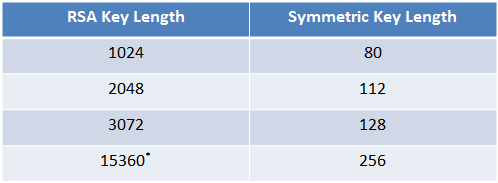
\includegraphics[width=0.7\textwidth]{figures/Strength_Equivalence.png}
        \caption[Strength Equivalence] {Strength Equivalence\cite{Kaliski2009}\cite{Publication2007}}
\end{figure}

RSA Security also claimed that 1024-bit keys are likely to become unsafe sometime between 2006 and 2010 while the 2048-bit keys are sufficient until 2030. Thus the RSA key length of 3072 bits will be required since 2030\cite{Kaliski2009}. RSA with 2048-bit or longer key should meet the requirement of file encryption key security of Secure Dropbox.

\subsection{Cryptographic Hash Function}

Cryptographic hash functions perform irreversible encryption on an arbitrary length plain text and returns a fixed length cipher. The hash digest is fixed for same input but tremendously changed as long as changes happen to content, no matter how trivial it is\cite{Merkle1990}. These one-way hash functions provide a rapid method for detecting any change made to the content and are also used for generating individual digest of content\cite{Merkle1990}. In web application context, user’s confidential information is usually stored in the form of hash digest in case of being exposed when server is exploited.

Since the hash function by definition has the same output with the same input, hash collision attack is easy to perform. For example: Alice sets her password as ``123456'' while Bob coincidentally sets his password as ``123456'' too. Consequently, same password hash values will be generated and stored. If Alice happens to get the password hash table that stored in the server, she might recognizes that Bob’s password hash value is exactly the same with hers and further realizes that Bob’s plain text password could be the same as Alice’s:

\begin{figure}[h]
        \centering
        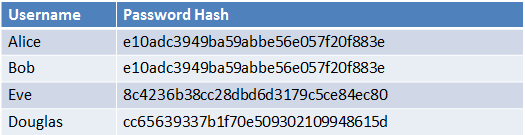
\includegraphics[width=0.8\textwidth]{figures/Hash_Table.png}
        \caption[Hash Table] {Hash Table}
\end{figure}

Also, if Alice has the dictionary of most frequently used password, she could try to hash each password in the collection and match to see if the same hash value exists. Accidentally she might find that Eve’s hashed password could be achieved by hashing ``654321'' with certain algorithm.

To protect the password hash value against hash collision attack, a random generated salt and configurable hash function iteration time could be applied when performing the content hashing. Randomly generated salt acts as a part of content to make same content distinct. The stored hash value is the result of hashing the combination of primary content and salt. Also the adoption of different iteration with different round times leads to a more sophisticated mapping relationship between plain text and hash value. The following example illustrates how a hash table with salt and iteration information stored in the server:

\begin{figure}[h]
        \centering
        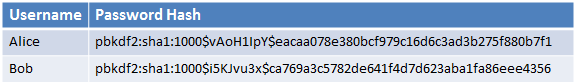
\includegraphics[width=0.9\textwidth]{figures/Hash_Table_with_Salt_Iteration_and_Algorithm_Indicated.png}
        \caption[Hash Table with Parameters] {Hash Table with Salt, Iteration and Algorithm Indicator}
\end{figure}

As shown above, there is additional information attached to the hash value. Take first record for example:

\begin{itemize}
  \item
  pdkdf2 indicates the library’s name via which the hash algorithm is used.
  \item
  sha1 indicates the algorithm used to generate the hash value.
  \item
  1000 indicates there are 1000 iterations when performing the password hashing.
  \item
  ``vAoH1lpY'' is the salt added to the plain text password before it is hashed.
\end{itemize}
		
The hash value to be matched should be generated with the above parameters. In this example, the SHA1 generates a 160-bit long digest of the content. It could be considered as a sufficient secure hash function since it is still widely used in mainstream security protocols like TLS and SSL.

\section {Integration with Dropbox}

Dropbox provides several kinds of APIs for Dropbox developers. For example, The Dropbox Core API, which is recommended as an ideal API set by Dropbox for server-based applications with programming interface for file reading and writing provided. It is also claimed as the most direct way to access Dropbox. Furthermore, it includes some advanced functionality interfaces like content search, version control and restoring file service for developers to performing low-level controls. The Dropbox Sync API, which provides file system-similar programming interface, encapsulates functionality implementations like synchronizing and notification of remote changes. It mainly orients to mobile platform programming. With respect to implementing Secure Dropbox, not only file synchronization operation like uploading and downloading, but also some low-level operations like file sharing, sharing URL generation and file metadata checking are required. To use Dropbox Core APIs, an access token obtained during Dropbox OAuth is essential. The access token will allows Secure Dropbox, a third-party application, to use the Dropbox API with granted permission but never get disclosed with any Dropbox user account information. The implementation details about how to perform the indirect authentication will be proposed in the implementation chapter. Some key Dropbox Core APIs are listed as follows:

\begin{figure}[h]
        \centering
        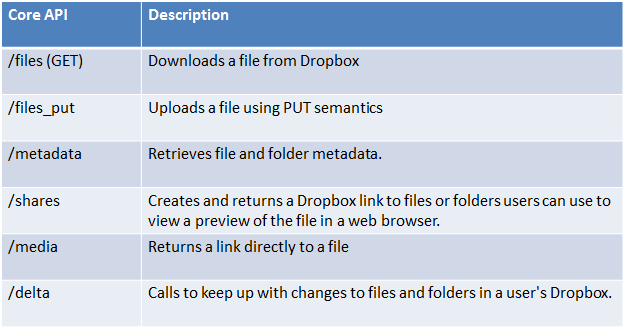
\includegraphics[width=0.9\textwidth]{figures/Key_Dropbox_Core_APIs_Functionality_Description.png}
        \caption[Dropbox Core API] {Key Dropbox Core APIs Functionality Description}
\end{figure}

Except exploiting these Dropbox APIs as advised, there is another way to use Dropbox service – synchronizing files through the Dropbox official application. Using Dropbox on the host computer is just like using any other folder in the file system. However, the files you drag or copy into Dropbox folder will be automatically synchronized and consequently synchronized to other terminals like mobile devices which are linked to Dropbox account. In this way, the Core API is still used but indirectly because the underlying interface for Dropbox official applications is implemented in Core API. The story with regard to file operation could be tremendously simplified if Secure Dropbox use the Dropbox client application as target folder and perform all file operations on it. Correspondingly, every encrypted file written into the Dropbox client folder will be uploaded automatically but without any Dropbox API invoked explicitly. A commercial software product with the same design and implementation relating to the hybrid usage of Dropbox APIs is Boxcryptor\cite{BoxCryptor2013}. Boxcryptor has a driver level encryption which is more efficient than user space encryption. However, the nature of client end encryption disables the sharing service infrastructures provided by Dropbox since file shared that way would be nonsense to human reader since the data is encrypted. Boxcryptor made their own sharing service which partially depends on Dropbox core API service like getting raw content of encrypted file via ``/media'' interface and sharing after decryption.

Although the Dropbox client folder eases the complexity when design the file operation module of Secure Dropbox, the file sharing feature of Dropbox client has been disabled. To analyze from API invoking’s perspective, ``/share'' function of Dropbox core API returns the URL refers to file or folder entity encapsulated with html information so there could be a rendered display of certain entity while the ``/media'' function returns the URL refers to a raw file content text. Apparently, if a file has been encrypted by Secure Dropbox and uploaded to Dropbox, it would be accessible by authenticated user but not meaningful until these encrypted data have been through the decryption service provided by Secure Dropbox. A potential solution to such a problem is a combination usage of Dropbox client and Dropbox API. For instance, the shared information could be accessed by firstly get the encrypted raw data via ``/media'' interface and decrypted in Secure Dropbox while other synchronization operations are still based on the Dropbox application. Another concern derives from the lack of access controls on Dropbox official application. The permission to use Dropbox application is incorrectly granted in the following scenario: Alice logins to Secure Dropbox service with her Secure Dropbox account and performs some file operations at her laptop. Bob comes to Alice and asks for a temporary use. When Bob logins with his Secure Dropbox account and uses Secure Dropbox, the file operations are actually performed on Alice’s Dropbox account. Dropbox does not open API to reset the Dropbox client account information of Dropbox application.

\section{C/S or B/S}

As so long as there is a cryptographic operation happens in the server end, there will be encryption key involved inevitably. It also potentially indicates that the server is allowed to do anything with the encryption key like storing or distributing it. So, to make Secure Dropbox security confident to users, KMS of Secure Dropbox will not be allowed to involve any cryptography procedure. Apparently a B/S architecture, where client is designed to be light while the server is fully responsible for all computations, will not be considered as a reasonable decision. It could be the foremost reason why a C/S designed architecture is more appropriate. However, to reduce the workload of server, in C/S architecture client is assigned with more tasks. Also only the processed data will be submitted to the server. Besides the key involvement issue, in Secure Dropbox the cryptography is the most resource consuming procedure especially when data to be processed is huge. All these tasks done by Secure Dropbox client end could significantly reduce the server’s workload. Based on this design, KMS’s work has been simplified to only process IO requests and perform local storage procedure. Where the encryption potentially involved in Secure Dropbox is illustrated as follows:

\begin{figure}[h]
        \centering
        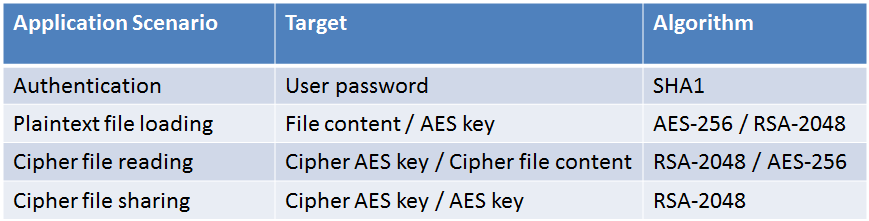
\includegraphics[width=0.9\textwidth]{figures/Cryptography_Application_Scenarios_in_Secure_Dropbox.png}
        \caption[Cryptography Deployment] {Cryptography Application Scenarios in Secure Dropbox}
\end{figure}







